\published{Journal of Geophysics and Engineering, 11, 045012, (2014)}

\title{Deblending using normal moveout and median filtering in common-midpoint gathers}

\renewcommand{\thefootnote}{\fnsymbol{footnote}}
\author{Yangkang Chen\footnotemark[1], Jiang Yuan\footnotemark[2], Zhaoyu Jin\footnotemark[3], Keling Chen\footnotemark[4] and Lele Zhang\footnotemark[5]}

\lefthead{Chen et al.}
\righthead{Deblending by NMO and \new{median filtering}\old{MF}}

\address{
\footnotemark[1]Bureau of Economic Geology, \\
Jackson School of Geosciences \\
The University of Texas at Austin \\
University Station, Box X \\
Austin, TX 78713-8924 \\
USA \\
%+1-5125478899 \\
ykchen@utexas.edu
%\ead{ykchen@utexas.edu}

\footnotemark[2] State Key Laboratory of Petroleum Resources and Prospecting \\
China University of Petroleum \\
Fuxue Road 18th\\
Beijing, China, 102200 \\

\footnotemark[3] School of Geosciences	\\
University of Edinburgh \\
%Grant Institute, The King's Buildings, West Mains Road \\
Edinburgh,UK, EH9 3JW \\

\footnotemark[4] Department of Earth and Atmospheric Sciences \\
University of Houston, \\
Houston, TX, 77004\\
USA \\
%kxc124930@gmail.com\\

\footnotemark[5]
Institute of Geology and Geophysics, \\
Chinese Academy of Sciences,\\
Beijing, China, 102200 \\
}

%\ead{ykchen@utexas.edu}

\begin{abstract}
The benefits of simultaneous source acquisition are compromised by the challenges of dealing with intense blending noise. In \old{the}\new{this} \old{abstract}\new{paper}, we propose a processing workflow \old{in the case of}\new{for} blended data. The incoherent property of blending noise in the common-midpoint \new{(CMP)} gather\new{s} is utilized for applying \old{a} median filter\new{ing} \new{along the spatial direction} \old{(MF)} after normal moveout (NMO) \new{correction}. The key \old{point}\new{step} in the proposed workflow is \old{the obtainment of}\new{that we need to obtain} a precise velocity \old{map}\new{estimation} which is required by the \old{following}\new{subsequent} NMO \new{correction}. \new{Because of the intense blending noise, the velocity scan can not be obtained in one step. We can recursively polish both deblended result and velocity estimation by deblending using the updated velocity estimation and velocity scanning using the updated deblended result.} 
We use synthetic and field data examples to \old{show}\new{demonstrate} the performance of the proposed approach\old{ and compare the final migrated images}. \new{The migrated image of deblended data is cleaner than that of blended data, and is similar to that of unblended data.}
\end{abstract}

%\newpage
%\maketitle
\section{Introduction}
The technique of simultaneous-source (sometimes called \emph{multisource}) acquisition means firing more than one shot\old{s} at nearly the same time regardless of their interference. \old{However, in}\new{In} conventional acquisition, \new{however,} either the temporal shooting intervals or the spatial sampling intervals are large enough so that the interference between successive shots can be \old{left out}\new{ignored}. \old{Thus, t}\new{T}he \old{novel}\new{multisource} technique can reduce the acquisition period and at the same time can improve \old{the} data quality because of the decreased spatial sampling interval \cite[]{berk}. The benefits from simultaneous-source acquisition are compromised by the challenges in removing strong blending interference.  Because of its economic benefits and technical challenges, this technique has attracted the attention of researchers in both industry and academia \cite[]{araz2011,mediandeblend}. 

In blended acquisition, more than one source \old{are}\new{is} shot simultaneously, regardless of their interactive interference. The term \emph{source} denotes a shot array, which can contain all the shots in a conventional acquisition system. When more than one source \old{are}\new{is} involved in acquisition, either a denser or a wider shot coverage can be obtained for a given constant acquisition period. Figure \ref{fig:demo1} \old{demonstrates}\new{depicts} two simultaneous sources shooting from the same position \old{to}\new{towards} the same direction. In this case, a two-times denser coverage can be obtained. Figure \ref{fig:demo2} \old{demonstrates}\new{depicts} two simultaneous sources far from each other shooting along the same direction, in which case, a two-times wider shot coverage can be obtained. The number of simultaneous sources can be even larger, \old{causing}\new{yielding} a much denser and wider shot coverage. The shooting sequence of the shots and the direction of each source can also be variable. \old{However, i}\new{I}t's natural\new{,} that the observed data will contain\old{s} strong interference, and the more simultaneous sources involved, the \old{stronger}\new{more severe} the interference will be. For the blended acquisition geometry as shown in Figure \ref{fig:demo2}\old{,} we \old{will} acquire \old{the} blended data\old{,} with strong interference, as shown in Figure \ref{fig:blenddemo}. Figure \ref{fig:datademo} shows the acquired data using conventional acquisition, suppos\old{ed}\new{ing} that the two sources in Figure \ref{fig:demo2} are fired with large-enough time interval.


\begin{figure}[htb!]
  \centering
% \subfigure[]{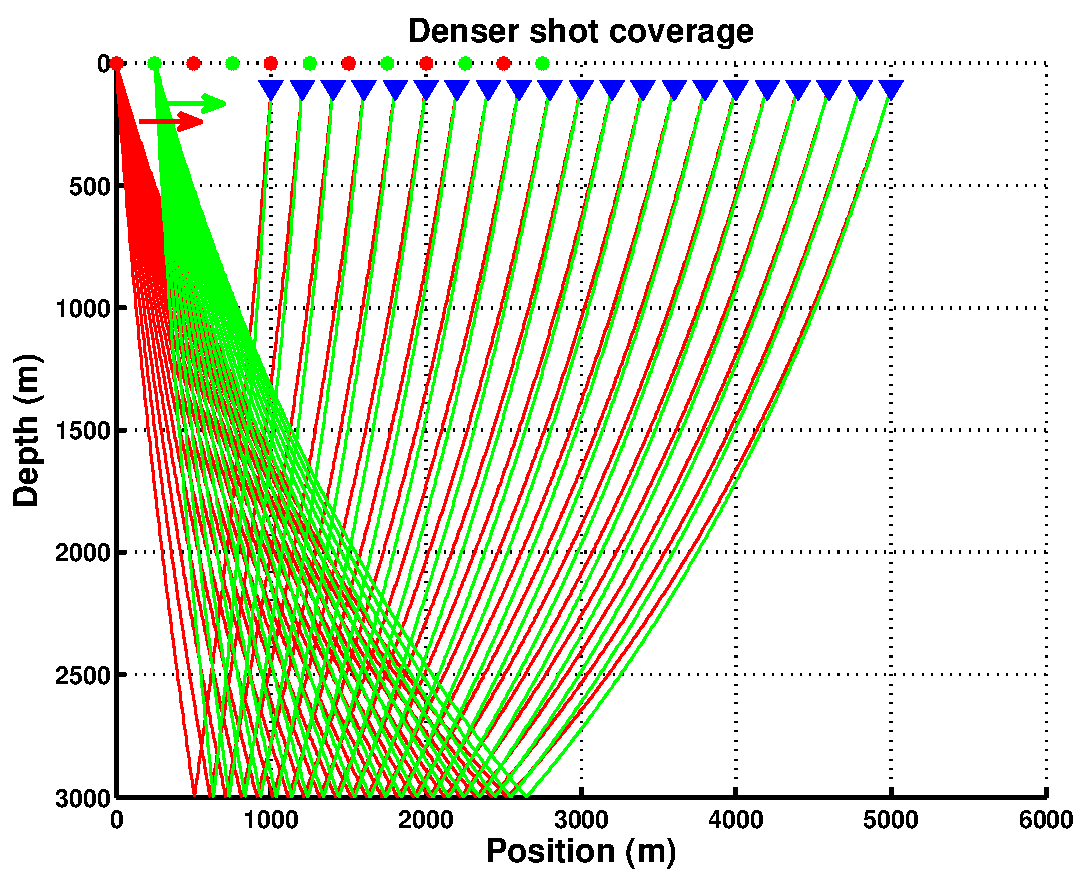
\includegraphics[width=0.485\columnwidth,height=0.45\columnwidth]{Fig/demo1}
 \subfigure[]{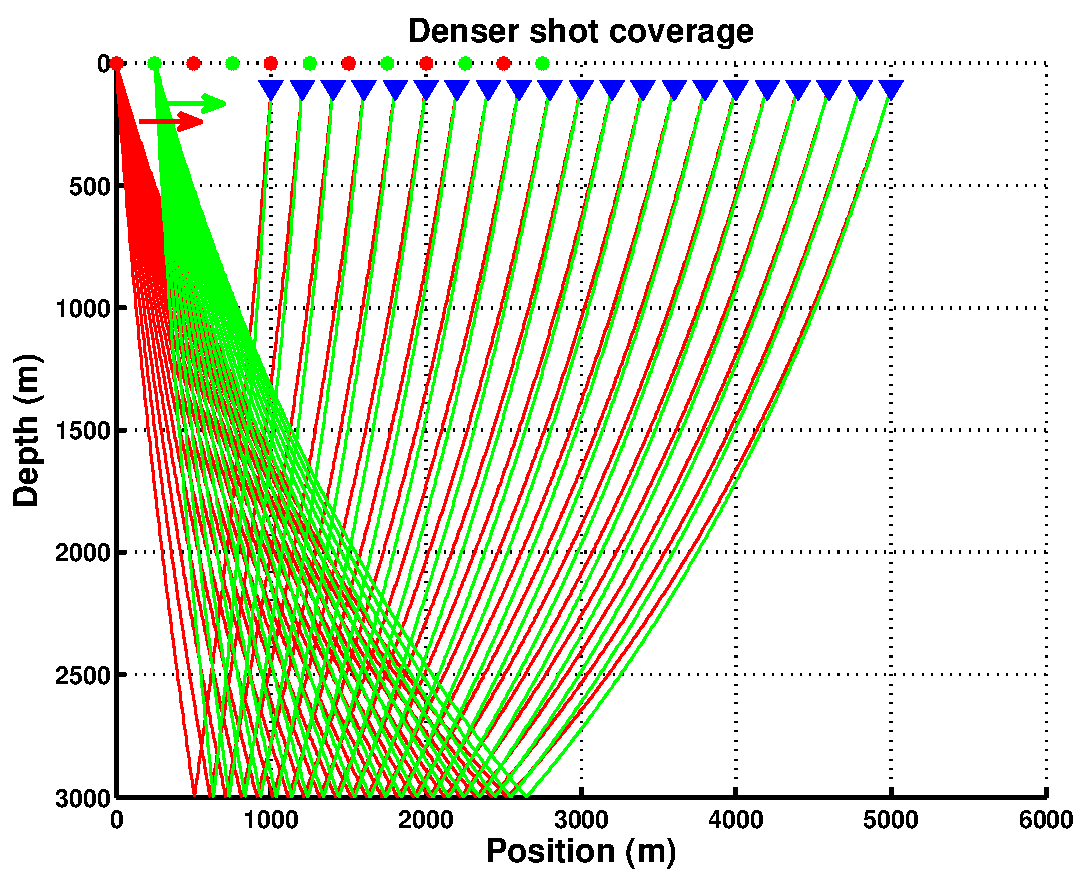
\includegraphics[width=\columnwidth,height=0.5\columnwidth]{Fig/demo1}
    \label{fig:demo1}}
%  \subfigure[]{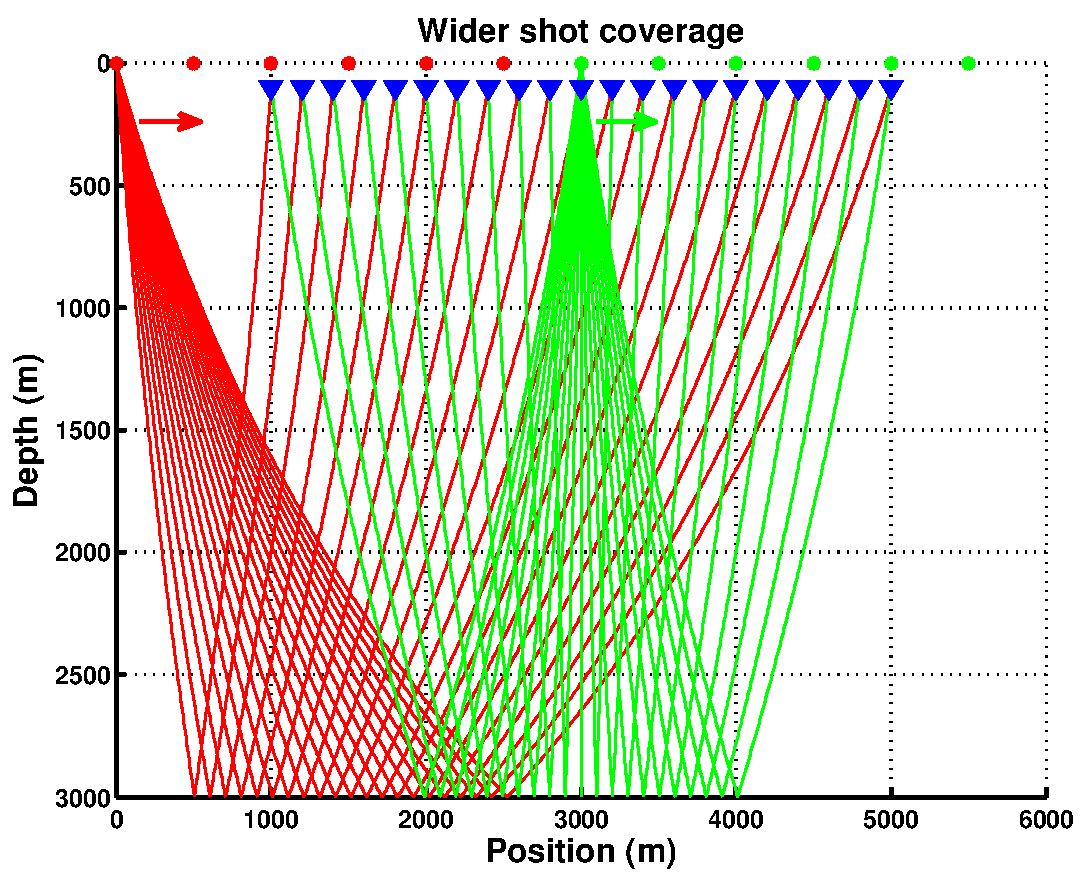
\includegraphics[width=0.485\columnwidth,height=0.45\columnwidth]{Fig/demo2}
  \subfigure[]{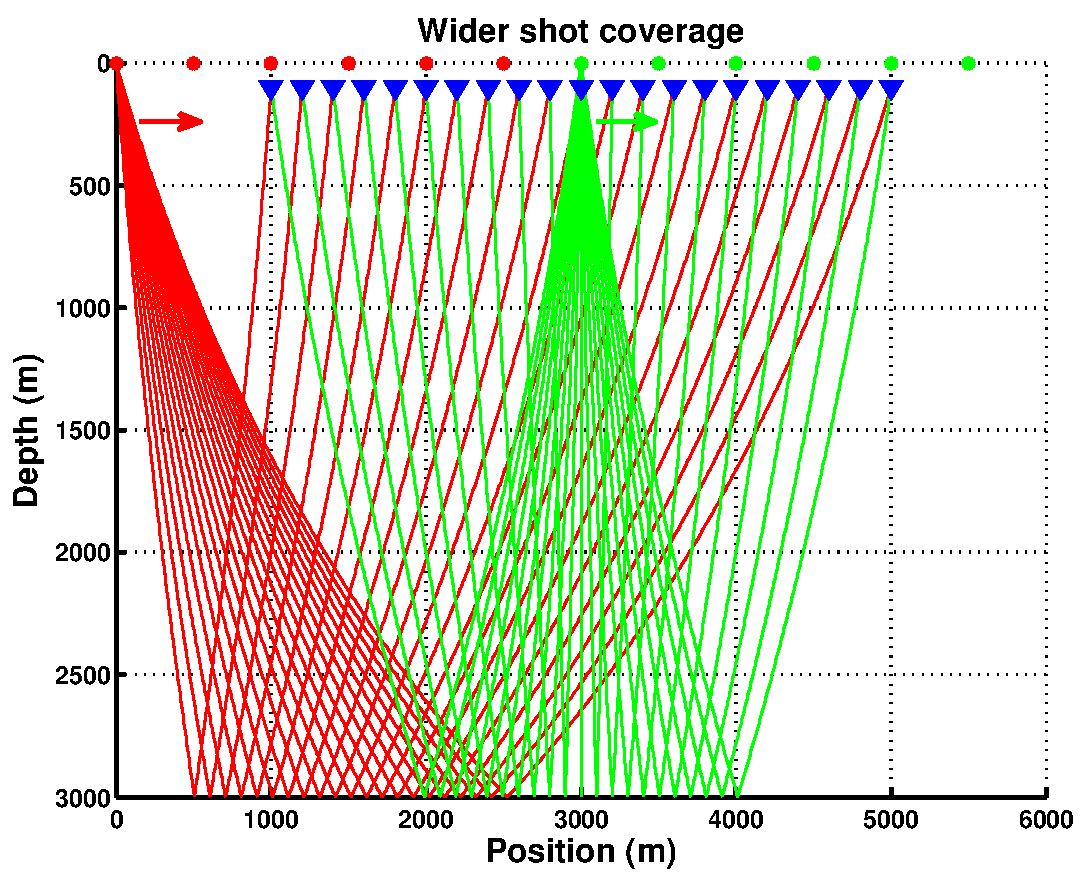
\includegraphics[width=\columnwidth,height=0.5\columnwidth]{Fig/demo2}
    \label{fig:demo2}}
   \caption{Demonstration for denser shot coverage (a) and wider shot coverage (b). Red points denote shot positions for source 1. Green points denote shot positions for source 2. Blue points denote receiver positions. Red and green strings denote the shooting rays. Arrows denote the shooting directions.} 
   \label{fig:demo1,demo2}%,sean-errorfk}
\end{figure}

\begin{figure}[htb!]
  \centering
% \subfigure[]{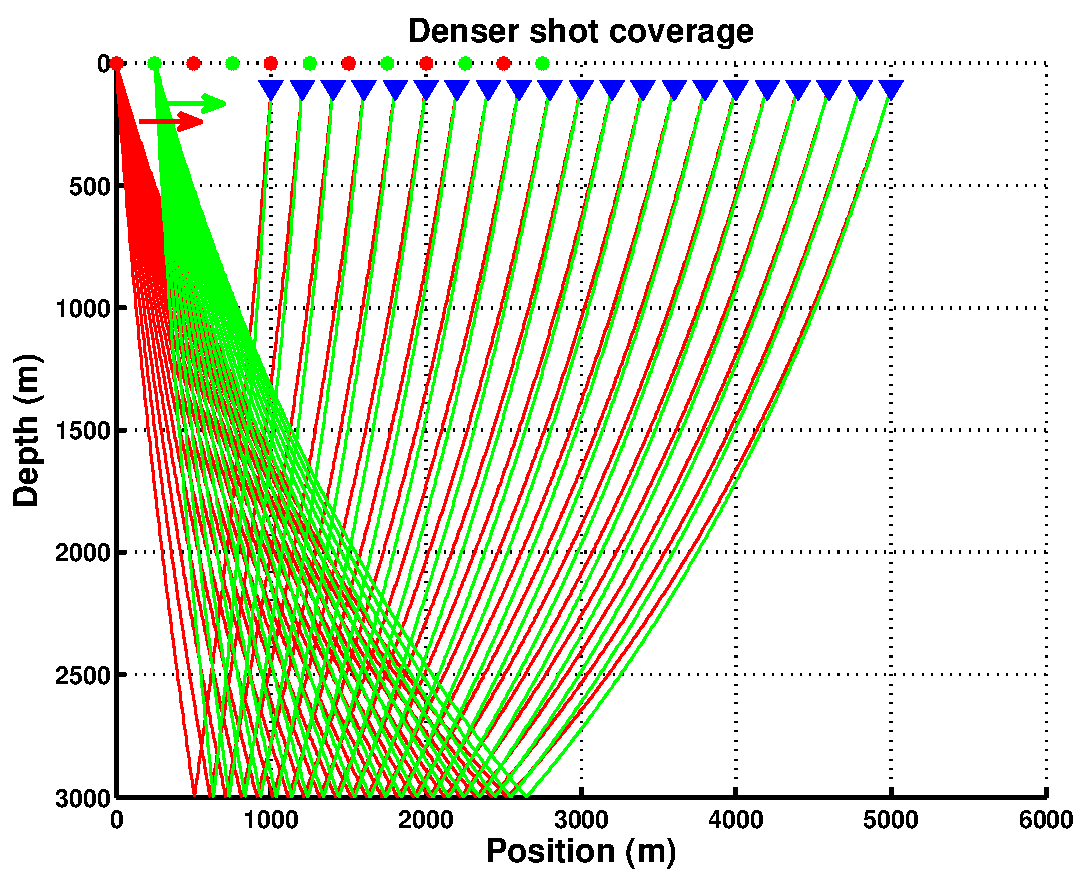
\includegraphics[width=0.485\columnwidth,height=0.45\columnwidth]{Fig/demo1}
 \subfigure[]{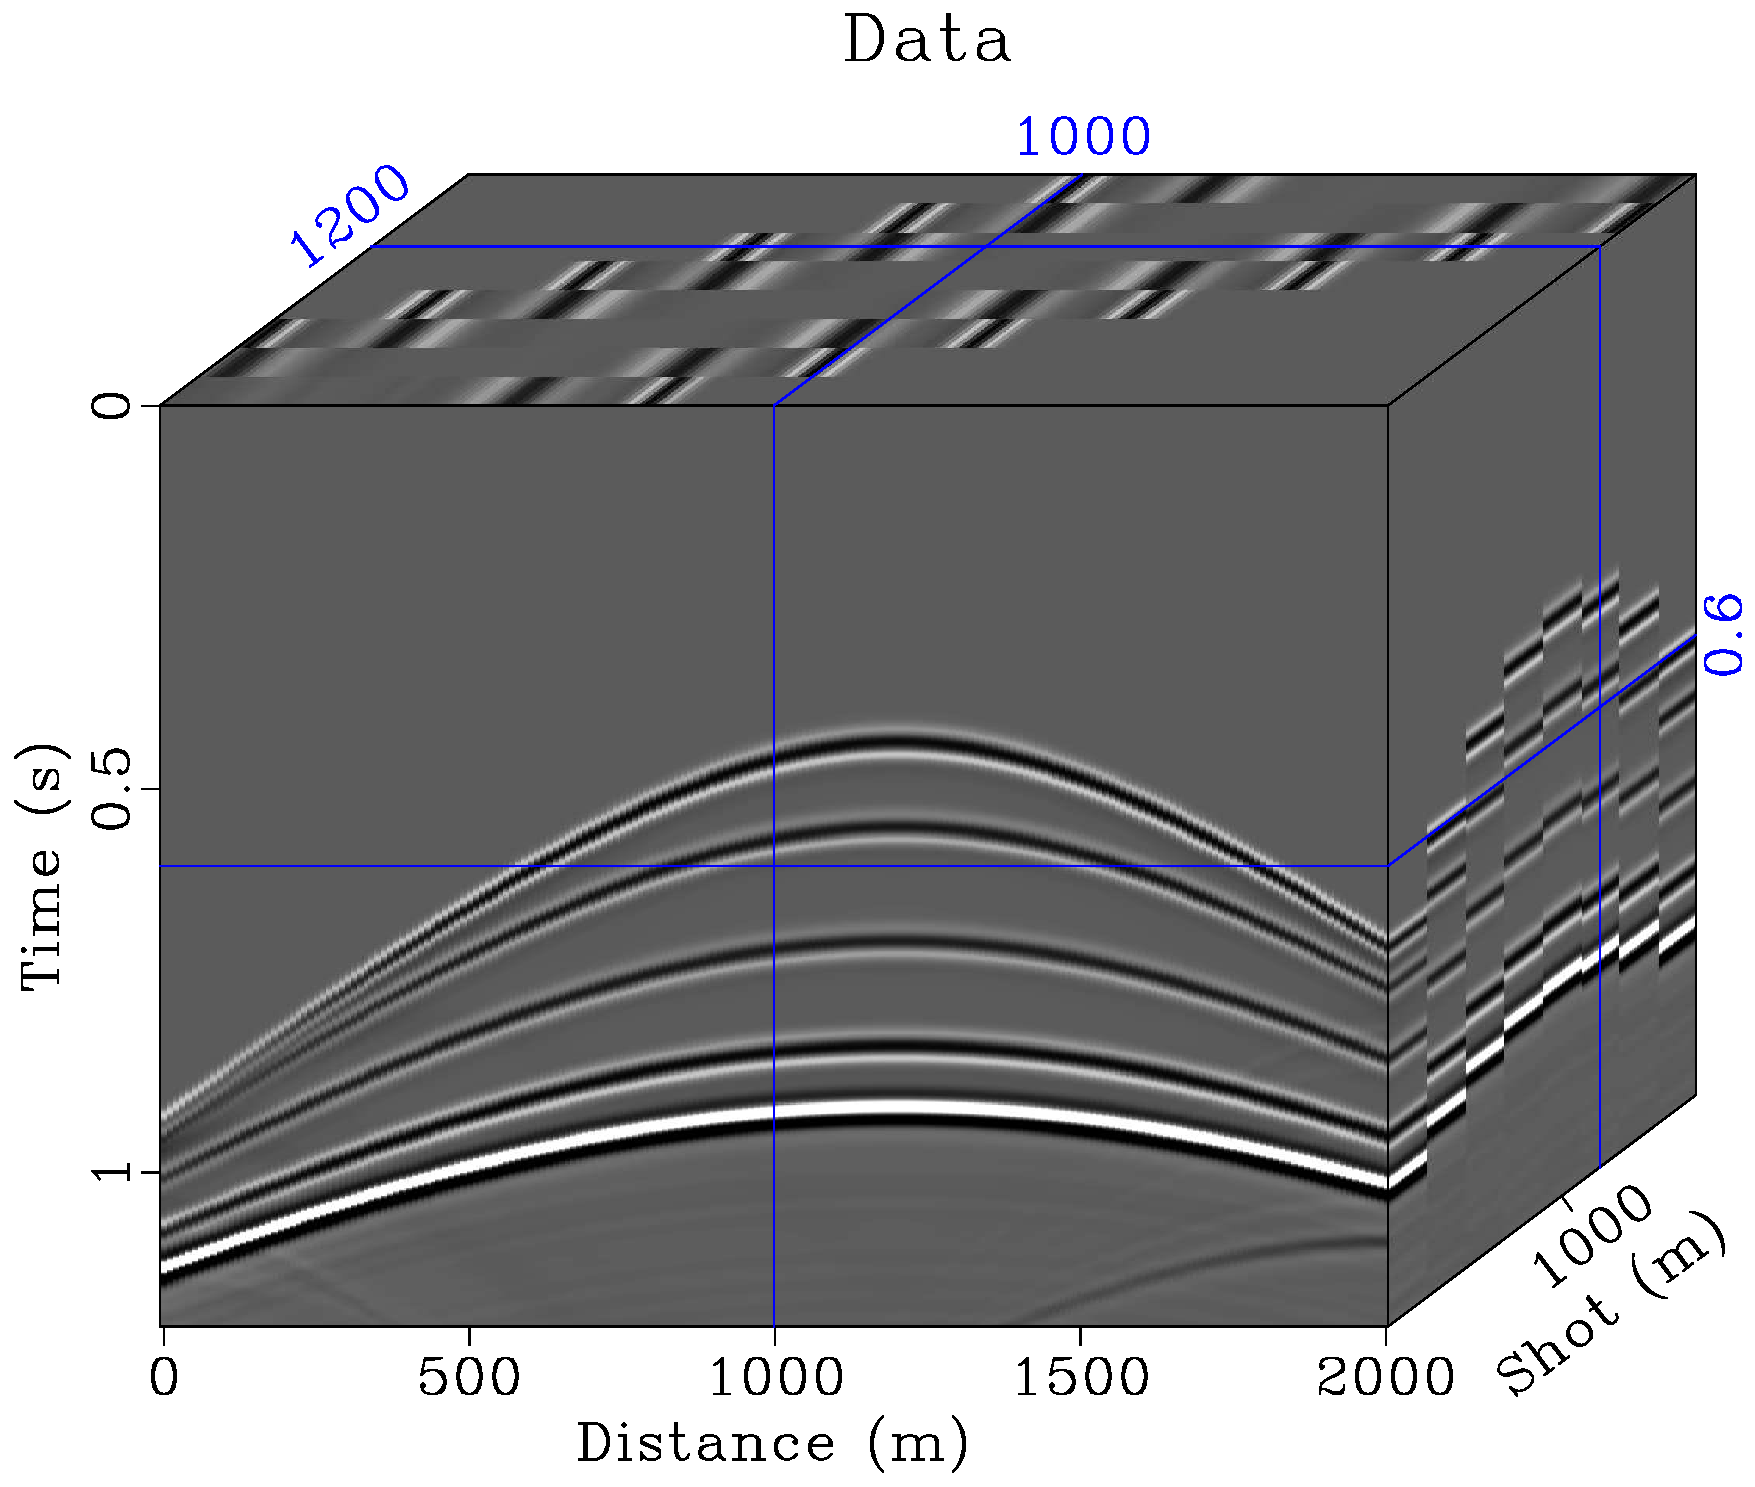
\includegraphics[width=0.485\columnwidth]{Fig/datademo}
    \label{fig:datademo}}
%  \subfigure[]{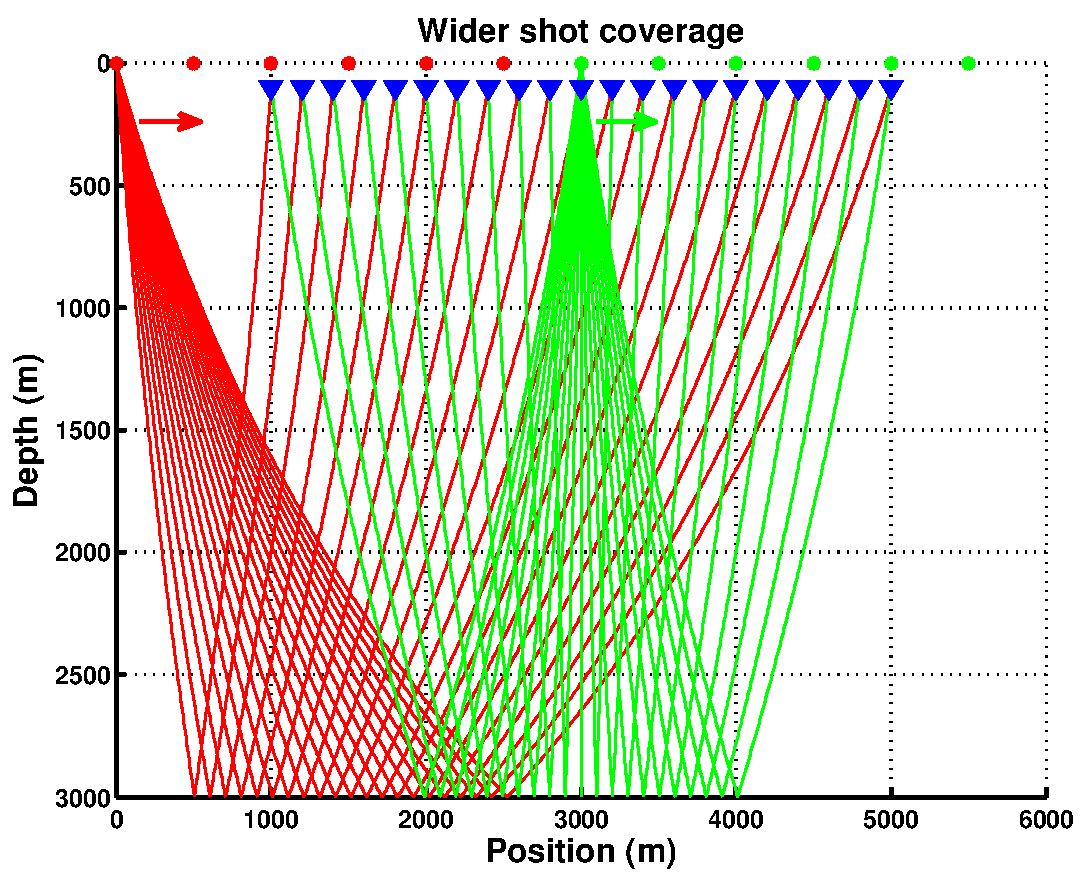
\includegraphics[width=0.485\columnwidth,height=0.45\columnwidth]{Fig/demo2}
  \subfigure[]{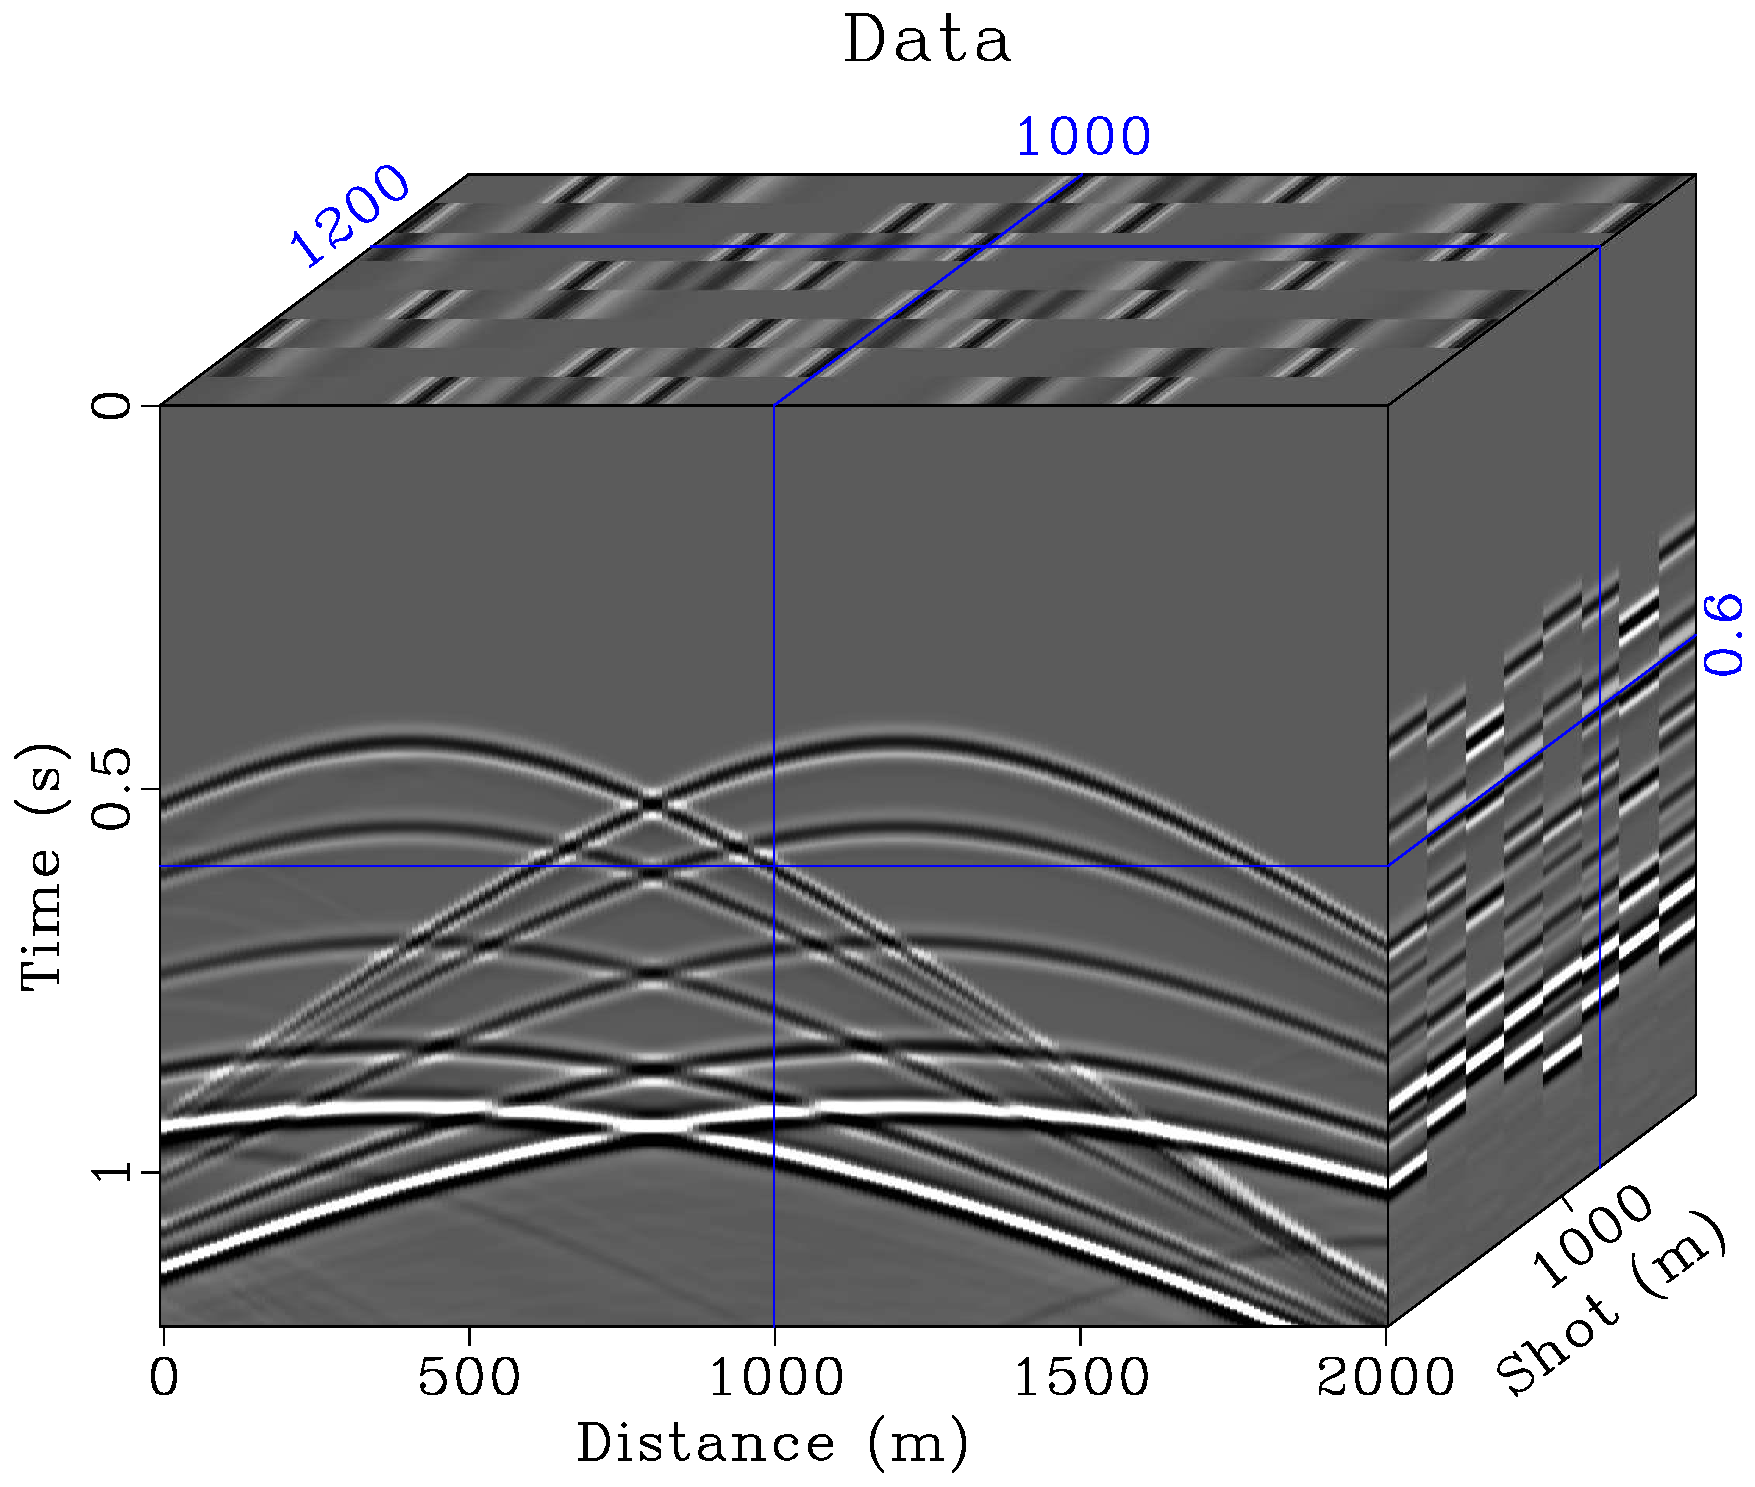
\includegraphics[width=0.485\columnwidth]{Fig/blenddemo}
    \label{fig:blenddemo}}
   \caption{(a) Unblended data. (b) Blended data.} 
   \label{fig:datademo,blenddemo}%,sean-errorfk}
\end{figure}

There are two main ways to deal with the challenges \old{set up}\new{posed} by simultaneous-source acquisition. The first \old{way} is \new{to use} \old{using} a first-separate and second-process strategy \cite[]{yangkang20131}, which is also known as "deblending" \cite[]{pana1}. The other is \new{to use}\old{using} direct imaging and waveform inversion by applying some constraint\new{s} to attenuate the artifacts caused by interference \cite[]{verschuur2011,daiwei2012}. Although the direct imaging approach has achieved some encouraging results, the preferable way \new{so far} is still \new{to} focus\old{ing} on the separation of blended data into individual \new{sources as if acquired conventionally}\old{ones}\new{.} \old{for the time being.}

%Other methods are based on improving

Different filtering and inversion methods have been used previously to deblend seismic data. Filtering methods utilize the property that the coherency of the simultaneous-source data is not the same in different domains, thus we can get the unblended data by filtering out the randomly distributed blending noise in \old{one special}\new{a particular} domain, \old{where}\new{in which} one source record is coherent and the other is not \cite[]{gary,araz2012,mediandeblend}. One choice is to transform seismic data from the common-shot domain to common-receiver, common-offset or common-midpoint domain. Inversion methods treat the separation problem as an estimation problem \old{which}\new{that} aims at estimating the desired \old{unknown} unblended data. Because of the ill-posed property of such estimation problems, a regularization term is usually required \cite[]{pana2}. \cite{moore2008}, \cite{akerberg2008} and \cite{moore2010} use a sparsity constraint in the Radon domain to regularize the inversion. A sparsity constraint is also used by \cite{abma2010} to minimize the energy of \old{the} incoherent events present in the blended data. \cite{bagaini2012} compared two separation techniques for \old{the} dithered slip-sweep (DSS) data using the sparse inversion method \cite{moore2010} and \old{the} $f$-$x$ predictive filtering \cite[]{canales1984,yangkang2014}, and \old{concluded}\new{found} \old{that} the advantage of \old{the} inversion methods over \old{the} random noise attenuation techniques. \cite{borselen2012} proposed to distribute all energy in the simultaneous shot records by reconstructing the individual shot records at their respective locations. \cite{araz2012} introduced an iterative estimation and subtraction scheme that combines the propert\old{y}\new{ies} of filtering and inversion methods and exploits the fact that\old{ the} characteristics of \old{the} blending noise differs in different domains. In order to deal with the aliasing problem, \cite{proj} proposed the alternating projection method (APM), which chooses corrective projections to exploit data characteristics and \old{is} claim\old{ed}\new{s} to be less sensitive to aliasing than \old{the} other approaches. 
%However, most of the published methods will either cause heavy signal leakage or cause large iterative computation. New efficient and robust deblending scheme is still demanded.

Median filter\new{ing} \old{(MF)} is \old{famous}\new{notable} for its ability \old{in}\new{to} remov\new{e}\old{ing} spiky noise and \old{thus} is \new{also} suitable \old{for removing}\new{to remove} blending noise. However, \new{median filtering}\old{MF} can \old{only} be applied \new{only} to seismic profile\new{s} containing horizontal events, otherwise it will harm much of the useful energy. In this \old{abstract}\new{paper}, we propose to implement \new{median filtering}\old{MF} to attenuate blending noise after normal moveout in common\new{-}midpoint (CMP) gather\new{s}. The deblending can be inserted into a \old{common}\new{conventional} processing workflow \old{where NMO velocity can be obtained}. The benefits of the proposed deblending approach are its easy implementation and \old{fast}\new{efficient} improvement for the migrated image without \new{use of} iterative deblending, which is extremely time-consuming. Synthetic and field data examples demonstrate the effectiveness of the deblending method and improvement for the final migrated image. 

\section{Method}
\subsection{Independent marine-streamer simultaneous shooting (IMSSS) }
As shown in Figure \ref{fig:streamer}, our blended survey is based on independent marine-streamer simultaneous shooting (IMSSS). Figure \ref{fig:streamer} shows four \old{indenpendent}\new{independent} marine-streamer sources. Note that the number of simultaneous sources \old{is}\new{need} not \new{be} limited to four. They shoot independently as \new{in} the conventional way and \old{get}\new{yield} their own data. For a 3D seismic survey, the IMSSS can help\old{s} \old{to} cover \old{the}\new{a} 2D surface area \old{much faster}\new{efficiently}. \old{In the case of}\new{With} four sources, the efficiency \old{can be}\new{is} increased by four times. \old{However, t}\new{T}he \old{tremendously} increased efficiency\new{, however,} is compromised by \old{the} interference among the four sources. \old{\new{In} \old{T}\new{t}he following sections we \old{will} introduce a simple but effective way to deal with the problem.}

\begin{figure}[htb!]
  \centering
% \subfigure[]{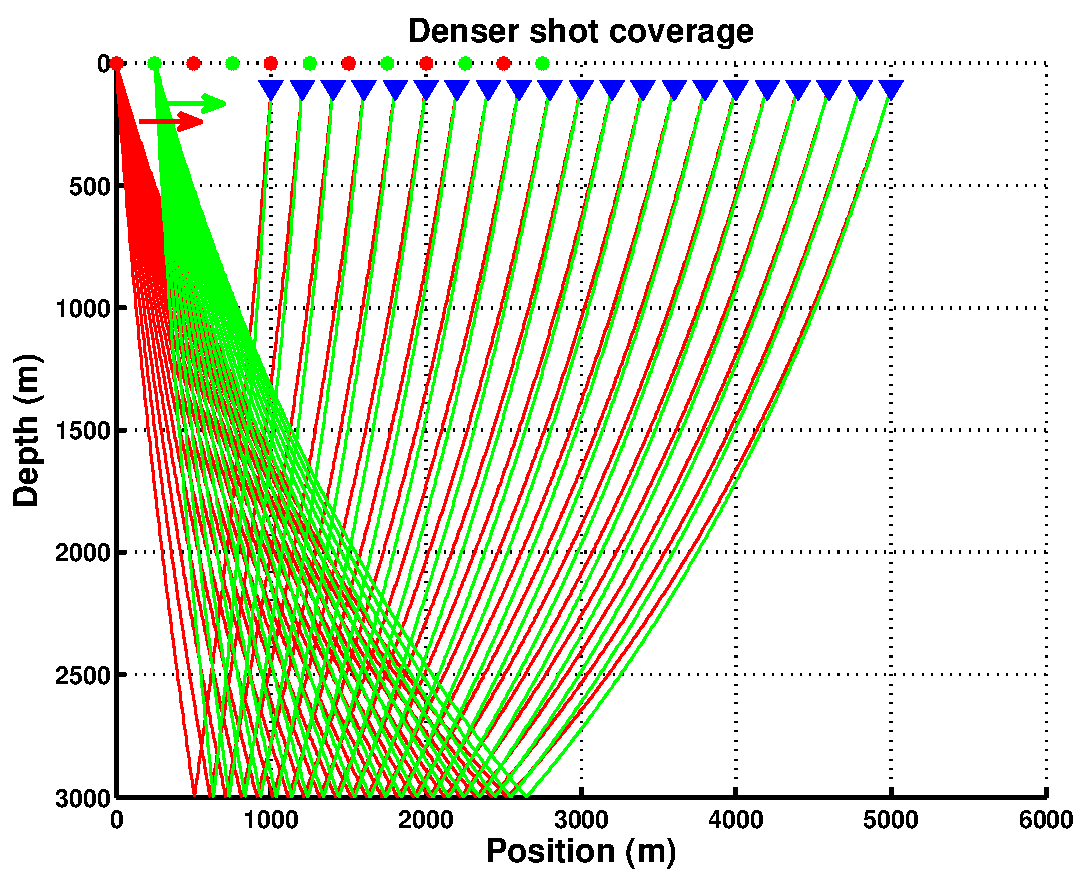
\includegraphics[width=0.485\columnwidth,height=0.45\columnwidth]{Fig/demo1}
 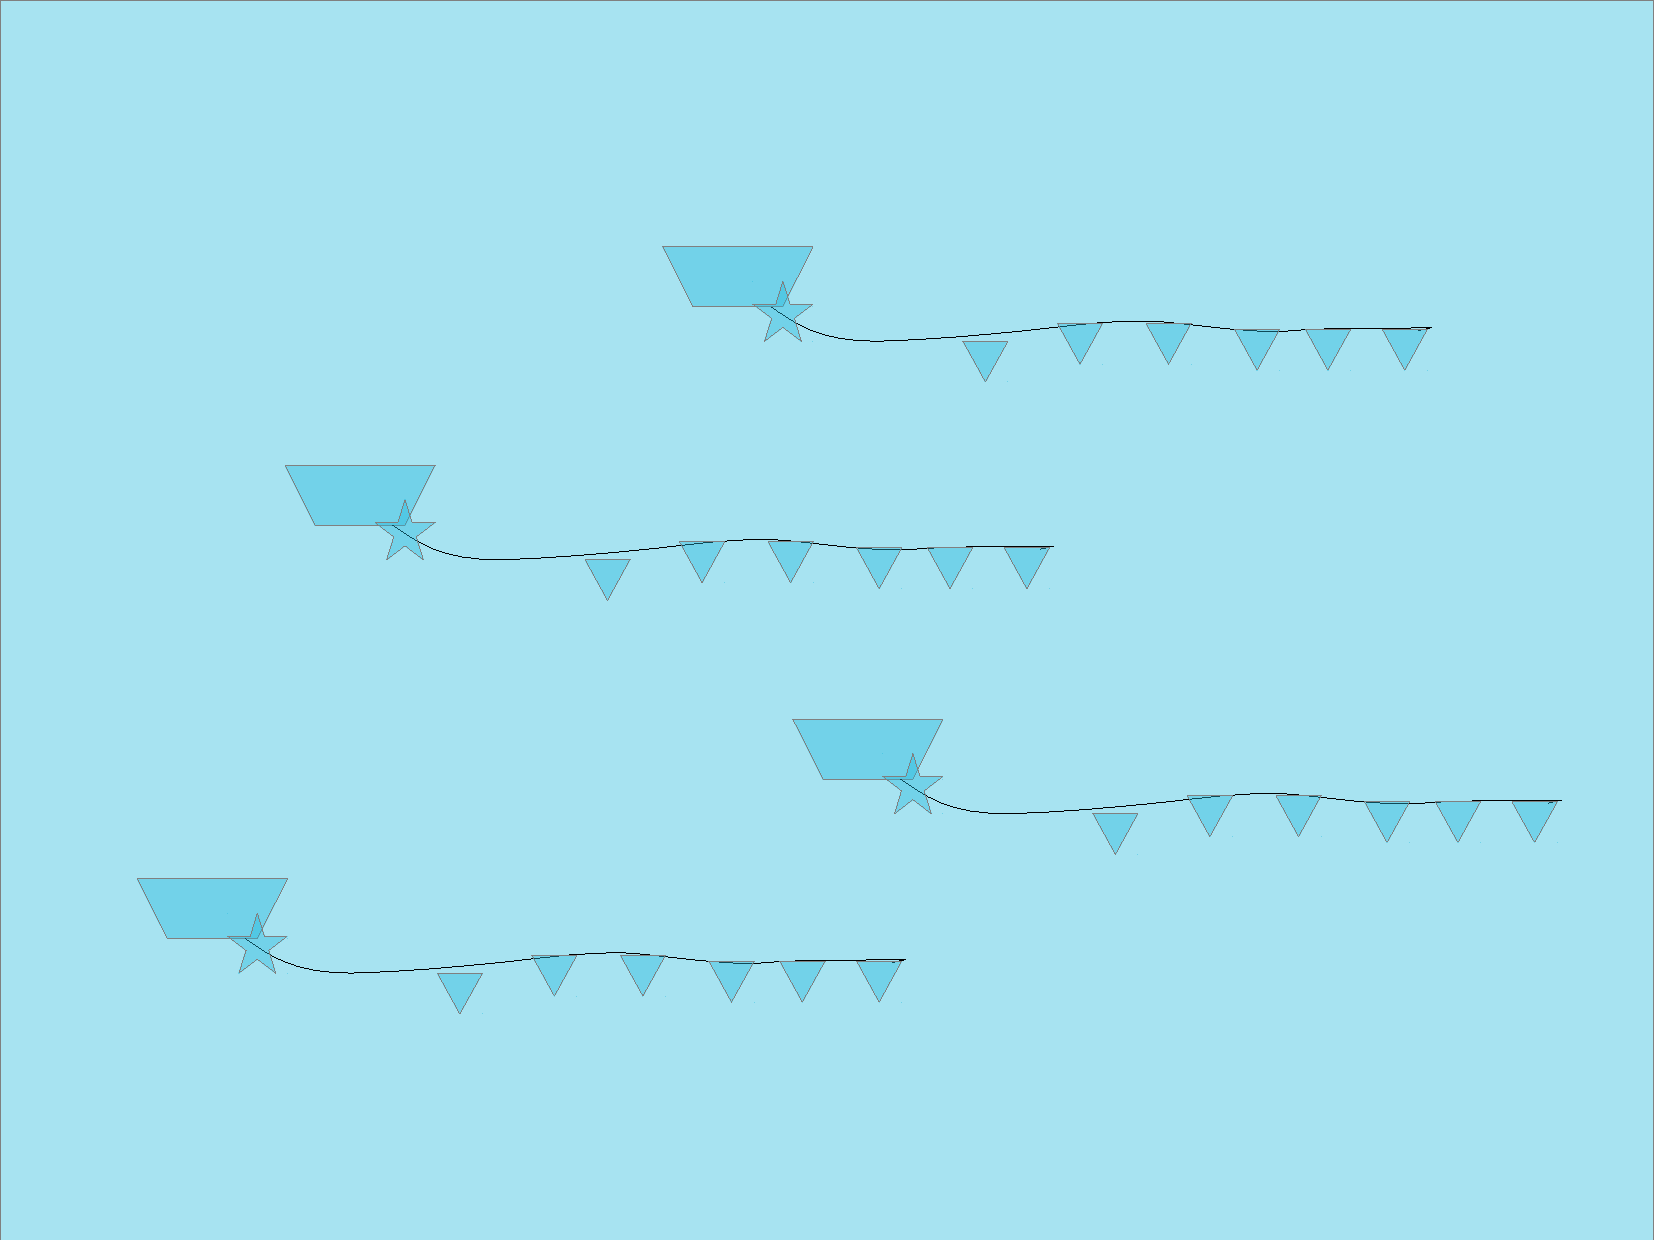
\includegraphics[width=\columnwidth,height=0.5\columnwidth]{Fig/streamer_demo}
   \caption{Demonstration \old{for}\new{of} independent marine-streamer simultaneous shooting (IMSSS).} 
    \label{fig:streamer}
\end{figure}

\subsection{Transformation between different domains}
The coherency of \old{the} simultaneous-source data is not the same in different domains. The interference appears coherent in common\new{-}shot gathers (CSG)\old{,}\new{;} however, the interference turns \new{out} to be incoherent when observed in common\new{-}midpoint gathers (CMG), common\new{-}offset gathers (COG) and common\new{-}receiver gathers (CRG).The transformation from shot-receiver domain to midpo\new{i}nt-half-offset domain can be realized by the following equations:



\begin{align}
\label{eq:trans1}
\mathbf{m} &= \frac{\mathbf{s}+\mathbf{r}}{2}, \\
\mathbf{h} &= \frac{\mathbf{r}-\mathbf{s}}{2},
\end{align}
where $\mathbf{m}$, $\mathbf{s}$ and $\mathbf{r}$ denote the coordinates of midpoint, shot\new{,} and receiver, respectively. $\mathbf{h}$ denotes the half\new{-}offset (with sign).

The transformation from shot-offset domain (\old{as }the acquired data from marine streamer) to midpoint-half-offset domain can be realized by the following equations:
\begin{align}
\label{eq:trans2}
\mathbf{m} &= \mathbf{s}+\frac{\mathbf{h}'}{2}, \\
\mathbf{h} &= \frac{\mathbf{h}'}{2},
\end{align}
where $\mathbf{h}'$ denotes the full offset.

Figure \ref{fig:data-csg} \old{demonstrates}\new{shows} \old{a }synthetic shot-offset domain unblended data simulated from marine-streamer acquisition. Figure \ref{fig:datas-csg} \old{demonstrates}\new{shows} the corresponding shot-offset\new{-}domain blended data using the IMSSS blended acquisition (with two sources). We can observe that the interference from \new{the} other source appears to be coherent in CSG. After transformation from \new{the} shot-offset domain to \new{the} midpoint-half-offset domain, the blending noise \old{turns into}\new{becomes} random \new{and} spike-like\new{,}\old{ noise,} as shown in Figure \ref{fig:datas-cmg}. Then deblending problem thus turns into a common denoising problem. Thus, in this section of examples, we focus on removing spiky noise in CMG. In the following sections, CSG also refers \new{to} the shot-offset domain and CMG also refers \new{to} the midpoint-half-offset domain. 

\begin{figure}[htb!]
\centering
\subfigure[]{\includegraphics[width=0.46\columnwidth]{class/Fig/data-csg.pdf}
\label{fig:data-csg}}
\subfigure[]{\includegraphics[width=0.46\columnwidth]{class/Fig/datas-csg.pdf}
\label{fig:datas-csg}}
\subfigure[]{\includegraphics[width=0.46\columnwidth]{class/Fig/data-b.pdf}
\label{fig:datas-cmg}}
\caption{(a) Unblended data in \new{the} shot-offset domain. (b) Blended data in \new{the} shot-offset domain. (c) Blended data in \new{the} midpoint-half-offset domain.}
\label{fig:data-csg,datas-csg,datas-cmg}
\end{figure}

\subsection{Median filter\new{ing}}
Conventional \new{median filtering}\old{MF} is based on a scalar-value sorting process. When a set of scalars is sorted \old{to be an}\new{into an} ascending or descending sequence, the middle value is chosen \old{to}\new{as} standard for this sequence. In signal-processing or geophysical data analysis fields, this filter is commonly used to remove spiky noise. The more general mathematical formulation of \old{a} \new{median filtering}\old{MF} is given as:
\begin{equation}
\label{eq:mf1}
\hat{u}_{i,j}=\arg\min_{u_m\in U_{i,j}}\sum_{l=1}^{L}\Arrowvert u_m-u_l \Arrowvert_p,
\end{equation}
where $\hat{u}_{i,j}$ is the output value for location $x_{i,j}$, $U_{i,j}=\{u_1,u_2,\cdots,u_L\}$, $i,j$ are the position indices in a 2-D profile, \new{and} $l$ and $m$ are both \old{a index}\new{indices} in the filtering window. $L$ is the length of the filtering window\new{,} and $p$ denotes $L_p$ norm. Commonly $p=1$ corresponds to \old{a} standard \new{median filtering}\old{MF}. 

Unlike 2D signal\old{-}processing \old{field}, where the signal is multi-dimensionally coherent, geophysical data \old{is}\new{are} only spatially \old{energy-focusing}\new{coherent}. \old{Due to}\new{Because of} the temporally sparse property, the useful signal \old{also} turns \old{to be}\new{into} a spike-like form. This spatial coherent characteristic\old{s} requires \old{a}\new{that} conventional \new{median filtering}\old{MF} \new{should} be taken along the spatial direction. \new{Here, spatial direction means the horizontal direction for a 2D seismic profile.} \old{Besides}\new{In addition}, the local slope of an event should be small in order to \old{ensure a small energy loss}\new{preserve more useful energy}. Figure \ref{fig:huos,huos-tmf,huos-xmf7,huos-xmf11} \old{demonstrate}\new{shows} the \old{effecitiveness}\new{effectiveness} of \old{a} \new{median filtering}\old{MF} in attenuating blending noise and preserving useful events\old{ in different cases}. Figure \ref{fig:huos-tmf} corresponds to \old{the} median filtering along \new{the} time direction with a filter length of 11. \old{By this way}\new{With this choice}, most of the useful energy has been removed. Figure \ref{fig:huos-xmf7} corresponds to median filtering along \old{space}\new{the spatial} direction with a filter length of 7. Figure \ref{fig:huos-xmf11} corresponds to median filtering along \old{space}\new{the spatial} direction with a filter length of 11. When the filter length is set \old{to be}\new{at} 7, most of horizontal energ\old{e}y is preserved and \old{a certained amount of}\new{some} dipping energy is lost. When the filter length is set \old{to be}\new{at} 11, most of the dipping energ\old{e}y is lost. Thus, we conclude that using \old{a} \new{median filtering}\old{MF} in \new{a profile with} dipping\old{-} events \old{profile} is dangerous\old{,}\new{;} \old{because }if the filter length is not appropriately chosen, the energy loss is heavy.

\old{In the case of}\new{For} dipping events, \old{a} multidimensional \new{median filtering}\old{MF} can be used as a substitute \cite[]{mediandeblend}\old{, otherwise \old{the} dipping events will be harmed seriously}. \old{However, a m}\new{M}ultidimensional \new{median filtering}\old{MF}\new{, however,} requires a precise estimation of the local slope of the seismic events, which may be difficult in field\new{-}data processing \old{because of}\new{in the presence of} \old{the} intense random or spiky noise. Besides, using \old{a} multidimensional \new{median filtering}\old{MF} needs much more computational cost and memory. \old{In this paper}\new{Here}, we propose \old{to use}\new{using} \new{median filtering}\old{MF} after NMO in the CMG, where the events are flatten and the effectiveness of \new{median filtering}\old{MF} is maximized.


\begin{figure}[htb!]
  \centering
% \subfigure[]{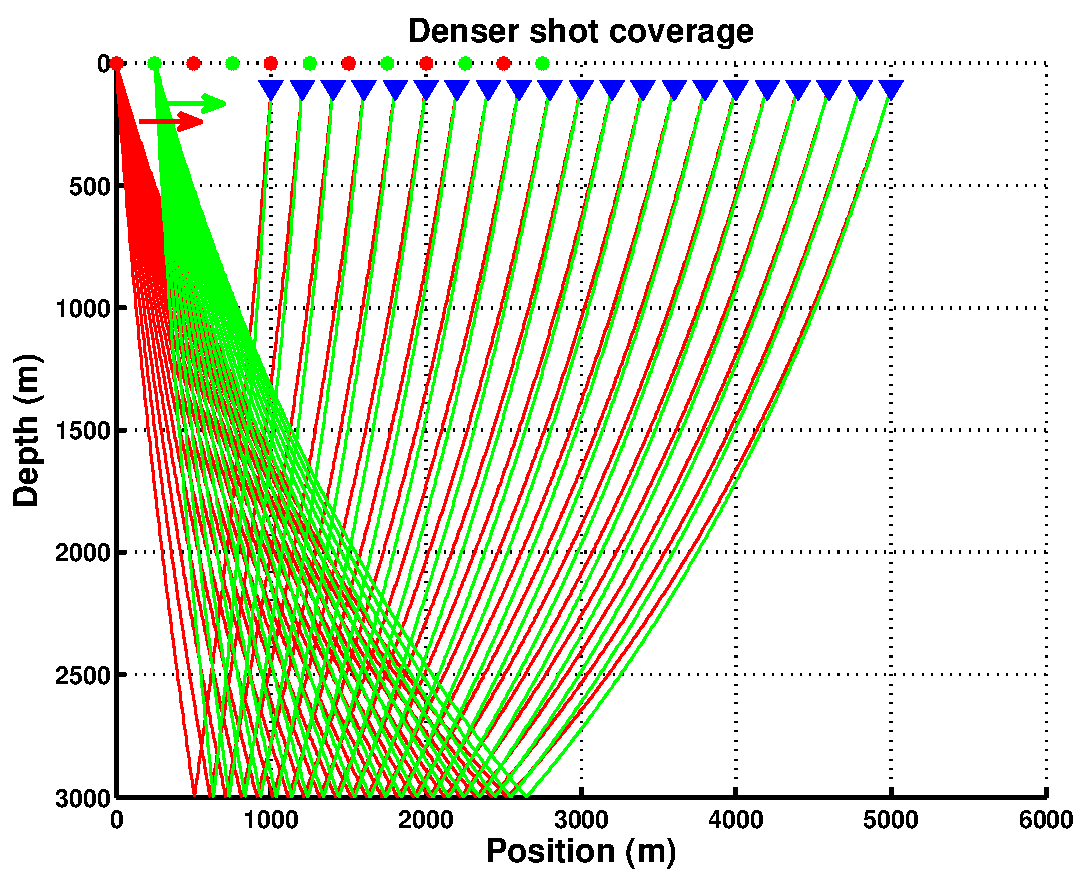
\includegraphics[width=0.485\columnwidth,height=0.45\columnwidth]{Fig/demo1}
 \subfigure[]{\includegraphics[width=0.485\columnwidth]{timespace/Fig/huos}
    \label{fig:huos}}
 \subfigure[]{\includegraphics[width=0.485\columnwidth]{timespace/Fig/huos-tmf}
    \label{fig:huos-tmf}}
 \subfigure[]{\includegraphics[width=0.485\columnwidth]{timespace/Fig/huos-xmf7}
    \label{fig:huos-xmf7}}
%  \subfigure[]{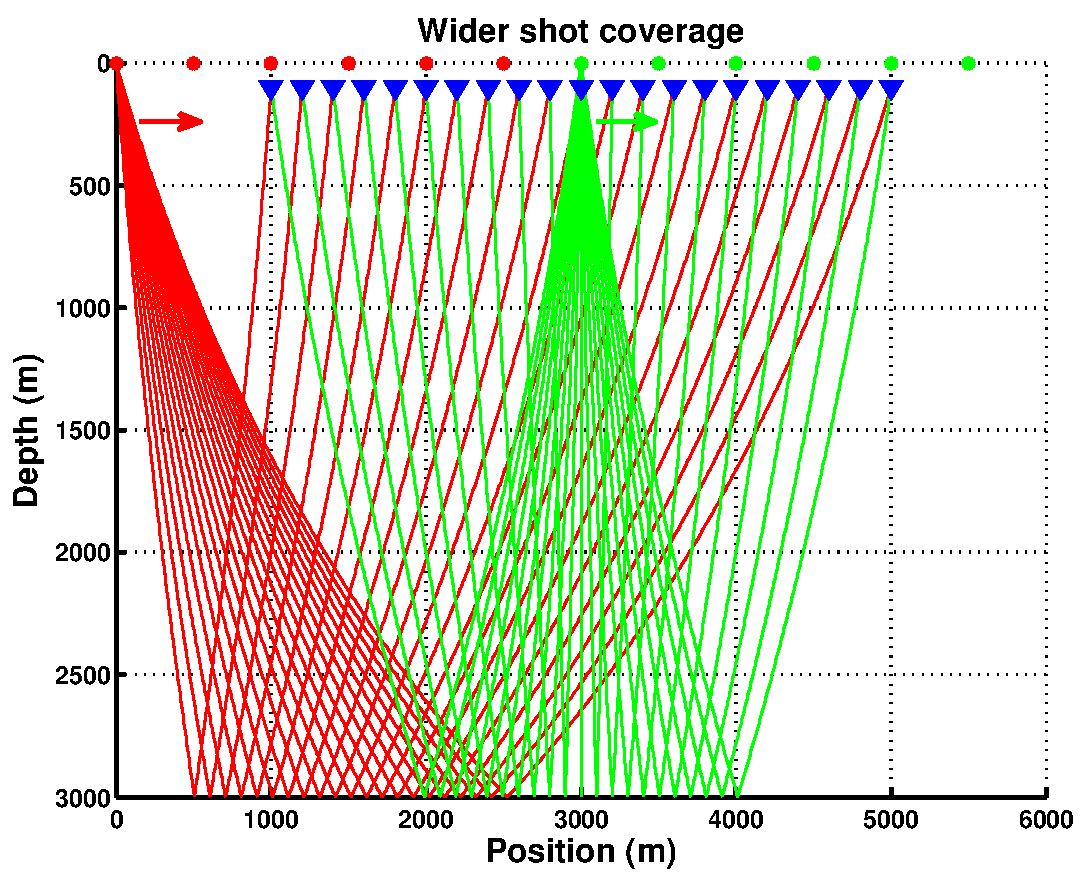
\includegraphics[width=0.485\columnwidth,height=0.45\columnwidth]{Fig/demo2}
  \subfigure[]{\includegraphics[width=0.485\columnwidth]{timespace/Fig/huos-xmf11}
    \label{fig:huos-xmf11}}
   \caption{(a) Blended data. (b) Median filtering along \new{the} time direction (filter length is 11). (c) Median filtering along space direction (filter length is 7). (d) Median filtering along space direction (filter length is 11). } 
   \label{fig:huos,huos-tmf,huos-xmf7,huos-xmf11}%,sean-errorfk}
\end{figure}

\subsection{Median filtering after NMO}
By utilizing the effectiveness of \new{median filtering}\old{MF} in removing spike-like noise and inserting \new{median filtering}\old{MF} into a common seismic processing workflow, we propose the following new processing workflow:
\begin{enumerate}
\item Transform the blended data from CSG to CMG.
\item \new{Apply} \old{V}\new{v}elocity scan and pick the NMO velocity.
\item \new{Apply} \old{N}\new{n}ormal moveout.
\item Apply median filtering along the offset direction in CMG.
\item \new{Apply} \old{I}\new{i}nverse normal moveout.
\item Prestack migration in CMG or transform back to CSG for other processing tasks. 
\end{enumerate}

The key point in the above workflow is flattening the seismic events in order to apply \old{a} \new{median filtering}\old{MF}, which results from obtaining a convincing velocity \old{spectrum}\new{scan}. Because of the intense blending noise, the velocity \old{spectrum}\new{scan} could not be obtained in one step. To solve the problem, we may need to implement steps 2-4 recursively\old{,} in order to get a better velocity \old{spectrum}\new{scan}. Two velocity scanning \old{is}\new{iterations are} usually adequate to get an acceptable velocity. \new{The proposed processing flow can recursively polish both deblended result and velocity estimation. On one hand, the better velocity estimation can help to make the NMO-corrected events flatter, which improve the performance of median filtering to remove blending noise and to preserve useful energy. On the other hand, the better deblended result can also help to improve the velocity estimation.}

\section{Examples}

\begin{figure}[htb!]
\centering
\subfigure[]{\includegraphics[width=0.46\columnwidth,height=0.600\columnwidth]{simple/Fig/cmpa.pdf}
\label{fig:cmpa}}
\subfigure[]{\includegraphics[width=0.46\columnwidth,height=0.600\columnwidth]{simple/Fig/cmp.pdf}
\label{fig:cmp}}
\subfigure[]{\includegraphics[width=0.46\columnwidth,height=0.600\columnwidth]{simple/Fig/semblancescn.pdf}
\label{fig:semblancescn}}
\caption{(a) Clean CMP gather. (b) Blended CMP gather. (c) Velocity scan for blended \old{cmp}\new{CMP} gather.}
\label{fig:cmpa,cmp,semblancescn}
\end{figure}

\begin{figure}[htb!]
\centering
\subfigure[]{\includegraphics[width=0.46\columnwidth,height=0.600\columnwidth]{simple/Fig/semblancenmo}
\label{fig:semblancenmo}}
\subfigure[]{\includegraphics[width=0.46\columnwidth,height=0.600\columnwidth]{simple/Fig/semblancenmomf}
\label{fig:semblancenmomf}}
\caption{(a) CMP gather after NMO. (b) CMP gather after NMO and median filtering.}
\label{fig:semblancenmo,semblancenmomf}
\end{figure}

\begin{figure}[htb!]
\centering
\subfigure[]{\includegraphics[width=0.46\columnwidth,height=0.600\columnwidth]{simple/Fig/semblanceinmo.pdf}
\label{fig:semblanceinmo}}
\subfigure[]{\includegraphics[width=0.46\columnwidth,height=0.600\columnwidth]{simple/Fig/semblancediffmf.pdf}
\label{fig:semblancediffmf}}
\subfigure[]{\includegraphics[width=0.46\columnwidth,height=0.600\columnwidth]{simple/Fig/semblanceerrormf.pdf}
\label{fig:semblanceerrormf}}
\caption{(a) CMP gathering after deblending. (b) Blending noise section. (c) Deblending error section.}
\label{fig:semblanceinmo,semblancediffmf,semblanceerrormf}
\end{figure}
The first example is a single synthetic CMP gather. The clean unblended data, blended data\new{,} and velocity scan of the blended data are shown in Figures \ref{fig:cmpa}, \ref{fig:cmp}\new{,} and \ref{fig:semblancescn}, respectively. Figure \ref{fig:semblancenmo,semblancenmomf} shows the blended data after NMO \new{correction} and deblended data after NMO \new{correction} and median filtering. The \new{median filtering}\old{MF} is effective in that \old{all}\new{most of} the interferences have been removed. After inverse NMO on Figure \ref{fig:semblancenmomf}, the deblended data in CMP gather is shown in Figure \ref{fig:semblanceinmo}. The blending noise section is shown in Figure \ref{fig:semblancediffmf}. From the deblending error section as shown in Figure \ref{fig:semblanceerrormf}, we conclude that the proposed method can achieve \old{perfect}\new{an excellent} result, because the deblending error is small.

We \old{next use}\new{now provide} two examples to demonstrate the performance of the proposed workflow described \old{in the previous content}\new{previously}. \new{In the next two examples, we use two sources to simulate the blended data.}
The second example is based on a simple synthetic dataset, which contains four reflectors. The velocity \new{in the} model is linearly increasing along the depth axis. We use Kirchhoff modeling to simulate the CSG and blend \old{them}\new{the data} according to IMSSS. After \old{a} common velocity\new{-}semblance scanning, we can pick the \old{normal moveout (NMO)}\new{NMO} velocity and \old{implement}\new{apply} NMO. \old{After a}\new{A}pplying \old{a} \new{median filtering}\old{MF} with a 9-point filter length along the offset direction\old{, we} remove\new{s} the blending noise. By inverse NMO, we get the deblended dataset in the common\new{-}midpoint domain.  Figure \ref{fig:data,data-b,data-db} shows the \old{comparison for}\new{comparison of} CMG\new{s}. Figure \ref{fig:vscan,vscan-b,vscan-db} shows the \old{comparison for}\new{comparison of} velocity scan, \old{from}\new{in} which we \old{find}\new{see} the velocity scan for the blended CMG is \old{nearly} smeared \old{in}\new{along with} the noise. \old{However, a}\new{A}fter scanning the \old{initially} deblended data \new{coming from the first rough velocity scan and first NMO correction}, we \old{can}\new{however} obtain a convincing velocity map. Using the updated NMO with new velocit\old{y}\new{ies}, we \old{may} get flatter events \old{which is}\new{that are} more suitable for median filtering.  Figure \ref{fig:pstm,pstm-b,pstm-db} shows the \old{comparison for}\new{comparison of} migrated images. \new{In this example, we use prestack kirchhoff time migration (PSKTM) \cite[]{docherty1991} as the migration operator. We then use Dix inversion \cite[]{dix1955} to convert the time image to depth image.} \old{It's obvious that t}\new{T}he migrated image after deblending is much cleaner than that of \new{the} blended data. 

The third example is a marine field dataset\old{, which comes } from the Gulf of Mexico. Figure \ref{fig:gulf,gulf-b,cmps-db} shows the \old{comparison for}\new{comparison of} CMG\new{s}. Figure \ref{fig:gulf-vscan,gulf-vscan-b,gulf-vscan-db} shows the \old{comparison for}\new{comparison of} velocity scan\new{s}. Figure \ref{fig:gulf-pstm,gulf-pstm-b,gulf-pstm-db} shows the \old{comparison for}\new{comparison of} \new{the} migrated image. \new{In this example, we use the same migration approach to obtain the seismic images.} We \old{can get}\new{have} the similar observation \new{to that for} \old{as} the second example\old{.}\new{:} \old{T}\new{t}he migrated image for the deblended data is cleaner, especially for the shallow part, indicated by the arrows \new{and frame boxes}. \new{For a better view, we zoom the parts indicated by frame boxes and show them in Figure \ref{fig:gulf-pstmzoom,gulf-pstm-bzoom,gulf-pstm-dbzoom}. It's obvious to see the improvement for the final migrated image after using the proposed deblending approach.}

\section{Conclusions}
We have proposed a basic workflow for dealing with blended data. The processing domain is in CMG, where blending noise appears to be incoherent and seismic reflection\new{s} \old{turns to be}\new{appear as} hyperbolic events. By applying \old{a common} \new{median filtering}\old{MF} \new{along the spatial direction} after NMO in CMG, we can easily remove the blending noise without harming useful signal. By applying inverse NMO, we can get the deblended data. \new{In order to obtain convincing velocity estimation, we use a recursive strategy. We polish both deblended result and velocity estimation by deblending using the updated velocity estimation and velocity scanning using the updated deblended result.} \old{The proposed deblending approach is efficient, without \new{the need for} any iteration process.} It is \old{also easy to be}\new{readily} implemented because we \old{only} use a conventional version of \new{median filtering}\old{MF} and don't use any other sophisticated technique to aid in the deblending process. The migrated image of the deblended data shows cleaner structure\new{ than that of blended data}, which \old{consolidates}\new{confirms the effectiveness of} the proposed deblending approach.

\section{Acknowledgments}
Yangkang Chen would like to thank FairfieldNodal for the opportunity for a summer internship. We also thank Sergey Fomel, Josef Paffenholz and Araz Mahdad for inspiring discussions and helpful suggestions. We \old{also} thank developers of Madagascar open-source platform for providing accessible codes.



\begin{figure}[htb!]
\centering
\subfigure[]{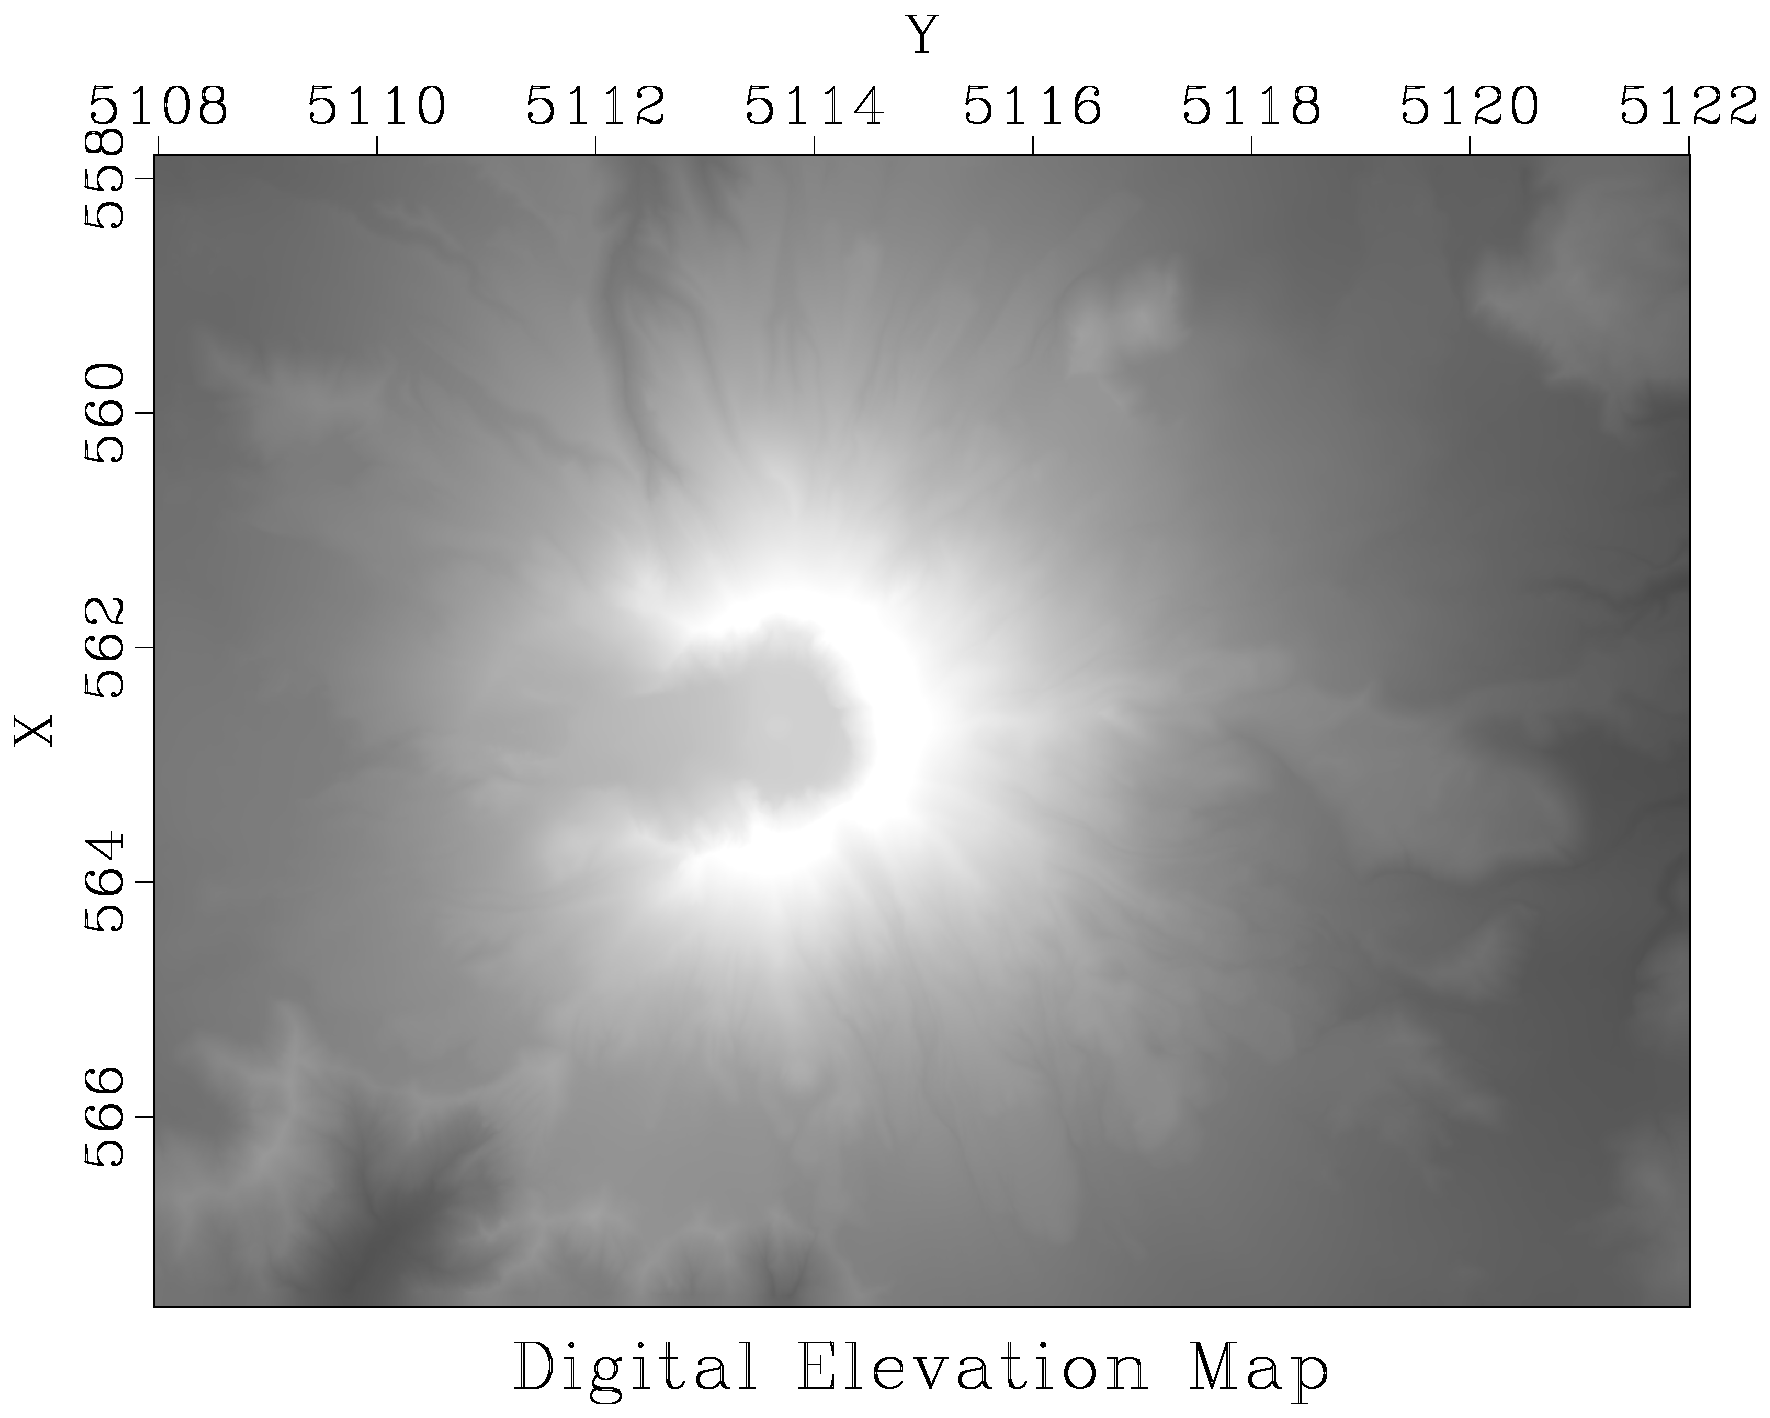
\includegraphics[width=0.46\columnwidth]{synth/Fig/data.pdf}
\label{fig:data}}
\subfigure[]{\includegraphics[width=0.46\columnwidth]{synth/Fig/data-b.pdf}
\label{fig:data-b}}
\subfigure[]{\includegraphics[width=0.46\columnwidth]{synth/Fig/data-db.pdf}
\label{fig:data-db}}
\caption{\old{Comparison for}\new{Comparison of} CMP gathers. (a) Original unblended CMP gathers. (b) Blended CMP gathers. (c) Deblended CMP gathers.}
\label{fig:data,data-b,data-db}
\end{figure}

\begin{figure}[htb!]
\centering
\subfigure[]{\includegraphics[width=0.46\columnwidth]{synth/Fig/vscan.pdf}
\label{fig:vscan}}
\subfigure[]{\includegraphics[width=0.46\columnwidth]{synth/Fig/vscan-b.pdf}
\label{fig:vscan-b}}
\subfigure[]{\includegraphics[width=0.46\columnwidth]{synth/Fig/vscan-db.pdf}
\label{fig:vscan-db}}
\caption{\old{Comparison for}\new{Comparison of} velocity scans. (a) Velocity scan for original unblended data. (b) Velocity scan for blended data. (c) Velocity scan for deblended data.}
\label{fig:vscan,vscan-b,vscan-db}
\end{figure}

\begin{figure}[htb!]
\centering
\subfigure[]{\includegraphics[width=0.46\columnwidth]{synth/Fig/pstm.pdf}
\label{fig:pstm}}
\subfigure[]{\includegraphics[width=0.46\columnwidth]{synth/Fig/pstm-b.pdf}
\label{fig:pstm-b}}
\subfigure[]{\includegraphics[width=0.46\columnwidth]{synth/Fig/pstm-db.pdf}
\label{fig:pstm-db}}
\caption{\old{Comparison for}\new{Comparison of} migrated images using prestack \old{k}\new{K}irchhoff time migration (PSKTM). (a) Migrated image for unblended data. (b) Migrated image for blended data. (c) Migrated image for deblended data.}
\label{fig:pstm,pstm-b,pstm-db}
\end{figure}

\begin{figure}[htb!]
\centering
\subfigure[]{\includegraphics[width=0.46\columnwidth]{bei/Fig/gulf.pdf}
\label{fig:gulf}}
\subfigure[]{\includegraphics[width=0.46\columnwidth]{bei/Fig/gulf-b.pdf}
\label{fig:gulf-b}}
\subfigure[]{\includegraphics[width=0.46\columnwidth]{bei/Fig/cmps-db.pdf}
\label{fig:cmps-db}}
\caption{\old{Comparison for}\new{Comparison of} CMP gathers. (a) Original unblended CMP gathers. (b) Blended CMP gathers. (c) Deblended CMP gathers.}
\label{fig:gulf,gulf-b,cmps-db}
\end{figure}

\begin{figure}[htb!]
\centering
\subfigure[]{\includegraphics[width=0.46\columnwidth]{bei/Fig/vscan-gulf.pdf}
\label{fig:gulf-vscan}}
\subfigure[]{\includegraphics[width=0.46\columnwidth]{bei/Fig/vscan-b.pdf}
\label{fig:gulf-vscan-b}}
\subfigure[]{\includegraphics[width=0.46\columnwidth]{bei/Fig/vscan-db.pdf}
\label{fig:gulf-vscan-db}}
\caption{\old{Comparison for}\new{Comparison of} velocity scans. (a) Velocity scan for original unblended data. (b) Velocity scan for blended data. (c) Velocity scan for deblended data.}
\label{fig:gulf-vscan,gulf-vscan-b,gulf-vscan-db}
\end{figure}

\begin{figure}[htb!]
\centering
\subfigure[]{\includegraphics[width=0.46\columnwidth]{bei/Fig/pstm.pdf}
\label{fig:gulf-pstm}}
\subfigure[]{\includegraphics[width=0.46\columnwidth]{bei/Fig/pstm-b.pdf}
\label{fig:gulf-pstm-b}}
\subfigure[]{\includegraphics[width=0.46\columnwidth]{bei/Fig/pstm-db.pdf}
\label{fig:gulf-pstm-db}}
\caption{\old{Comparison for}\new{Comparison of} migrated images using prestack \old{k}\new{K}irchhoff time migration (PSKTM). (a) Migrated image for unblended data. (b) Migrated image for blended data. (c) Migrated image for deblended data.}
\label{fig:gulf-pstm,gulf-pstm-b,gulf-pstm-db}
\end{figure}

\begin{figure}[htb!]
\centering
\subfigure[]{\includegraphics[width=0.46\columnwidth]{bei/Fig/pstmzoom.pdf}
\label{fig:gulf-pstmzoom}}
\subfigure[]{\includegraphics[width=0.46\columnwidth]{bei/Fig/pstm-bzoom.pdf}
\label{fig:gulf-pstm-bzoom}}
\subfigure[]{\includegraphics[width=0.46\columnwidth]{bei/Fig/pstm-dbzoom.pdf}
\label{fig:gulf-pstm-dbzoom}}
\caption{\old{Comparison for}\new{Comparison of} zoomed migrated images using prestack \old{k}\new{K}irchhoff time migration (PSKTM). (a) Zoomed migrated image for unblended data. (b) Zoomed migrated image for blended data. (c) Zoomed migrated image for deblended data.}
\label{fig:gulf-pstmzoom,gulf-pstm-bzoom,gulf-pstm-dbzoom}
\end{figure}

\bibliographystyle{seg}
\bibliography{nmo}







